\section{Dataset}
\label{sec:data}
Although there are many currently available dialogue datasets, 
most of them are used for training automatic dialogue robots/systems, 
thus don't have diversity in the speakers personal relationships or 
the relationship labels are hardly available.
Therefore, we build a new dataset 
composed of $6,307$ sessions of dyadic dialogues with labels 
about the personal relationship between the two speakers, 
starting from movie scripts crawlled from 
The Internet Movie Script Database (IMSDb).
%~\footnote{\url{https://www.imsdb.com/}}.

\subsection{Movie Dialogues vs. Real-world Dialogues}
Recording real-life dialogues, especially those of various relationships, 
is really hard to be carried out on large scale. Therefore, in this paper,
we instead use movie dialogues, which is abundant and 
easy to process computationally. 
Whether movie dialogues are good substitutes for 
real-world ones can be debatable. 
A previous study focusing on language entrainments~\cite{cornell-corpus} 
also build their conversation dataset from movie scripts. 
They find that movie dialogues exhibit stylistic convergence 
similar to real-world ones. Livingstone~\shortcite{television} states in 
the book \textit{Making Sense of Television: The Psychology of 
Audience Interpretation} that television contents and real-life experiences, 
despite their physical difference, are perceived through the same, 
or at least, heavily overlapping, interpretative frameworks. 
We thus make the reasonable assumption that humans employ 
similar knowledge and intuition when making inferences about the 
relationship of speakers from movie dialogues as from real-world ones.

\subsection{Dialogue Extraction and Processing}
Initially, we crawl 995 movie scripts from IMSDb, and 941 remain after 
we automatically match the titles with movies in 
IMDb\footnote{\url{https://www.imdb.com/}} and filter out those that 
(1) don't have a match in IMDb; (2) are not in english; 
(3) are very unpopular(measured by number of raters). 
By observing the formats of the scripts and manually defining text patterns, 
we split each script into scenes, extract the sequence of (speaker, utterance) 
pairs for each scene and identify subsequences that meet the following requirements  
as dyadic dialogue sessions: 
(1) two speakers speak alternately without being interrupted 
by a third one; 
(2) each contains at least 3 turns. 
We set this minimum length requirement to make sure 
that two speakers are speaking to each other instead of 
participating in a group discussion. 
Finally, we count total number of turns taken 
between each character pairs and filter out those having 
fewer than 20 turns to 
make sure the relationship between the two characters is significant 
and not as trivial as greetings between strangers. 
This filtering step also helps reduce the cost of labeling 
because more sessions can share the same pair of speakers.

\subsection{Labeling Methodology}
\subsubsection*{The Taxonomy}
\begin{figure}[th]
	\centering
	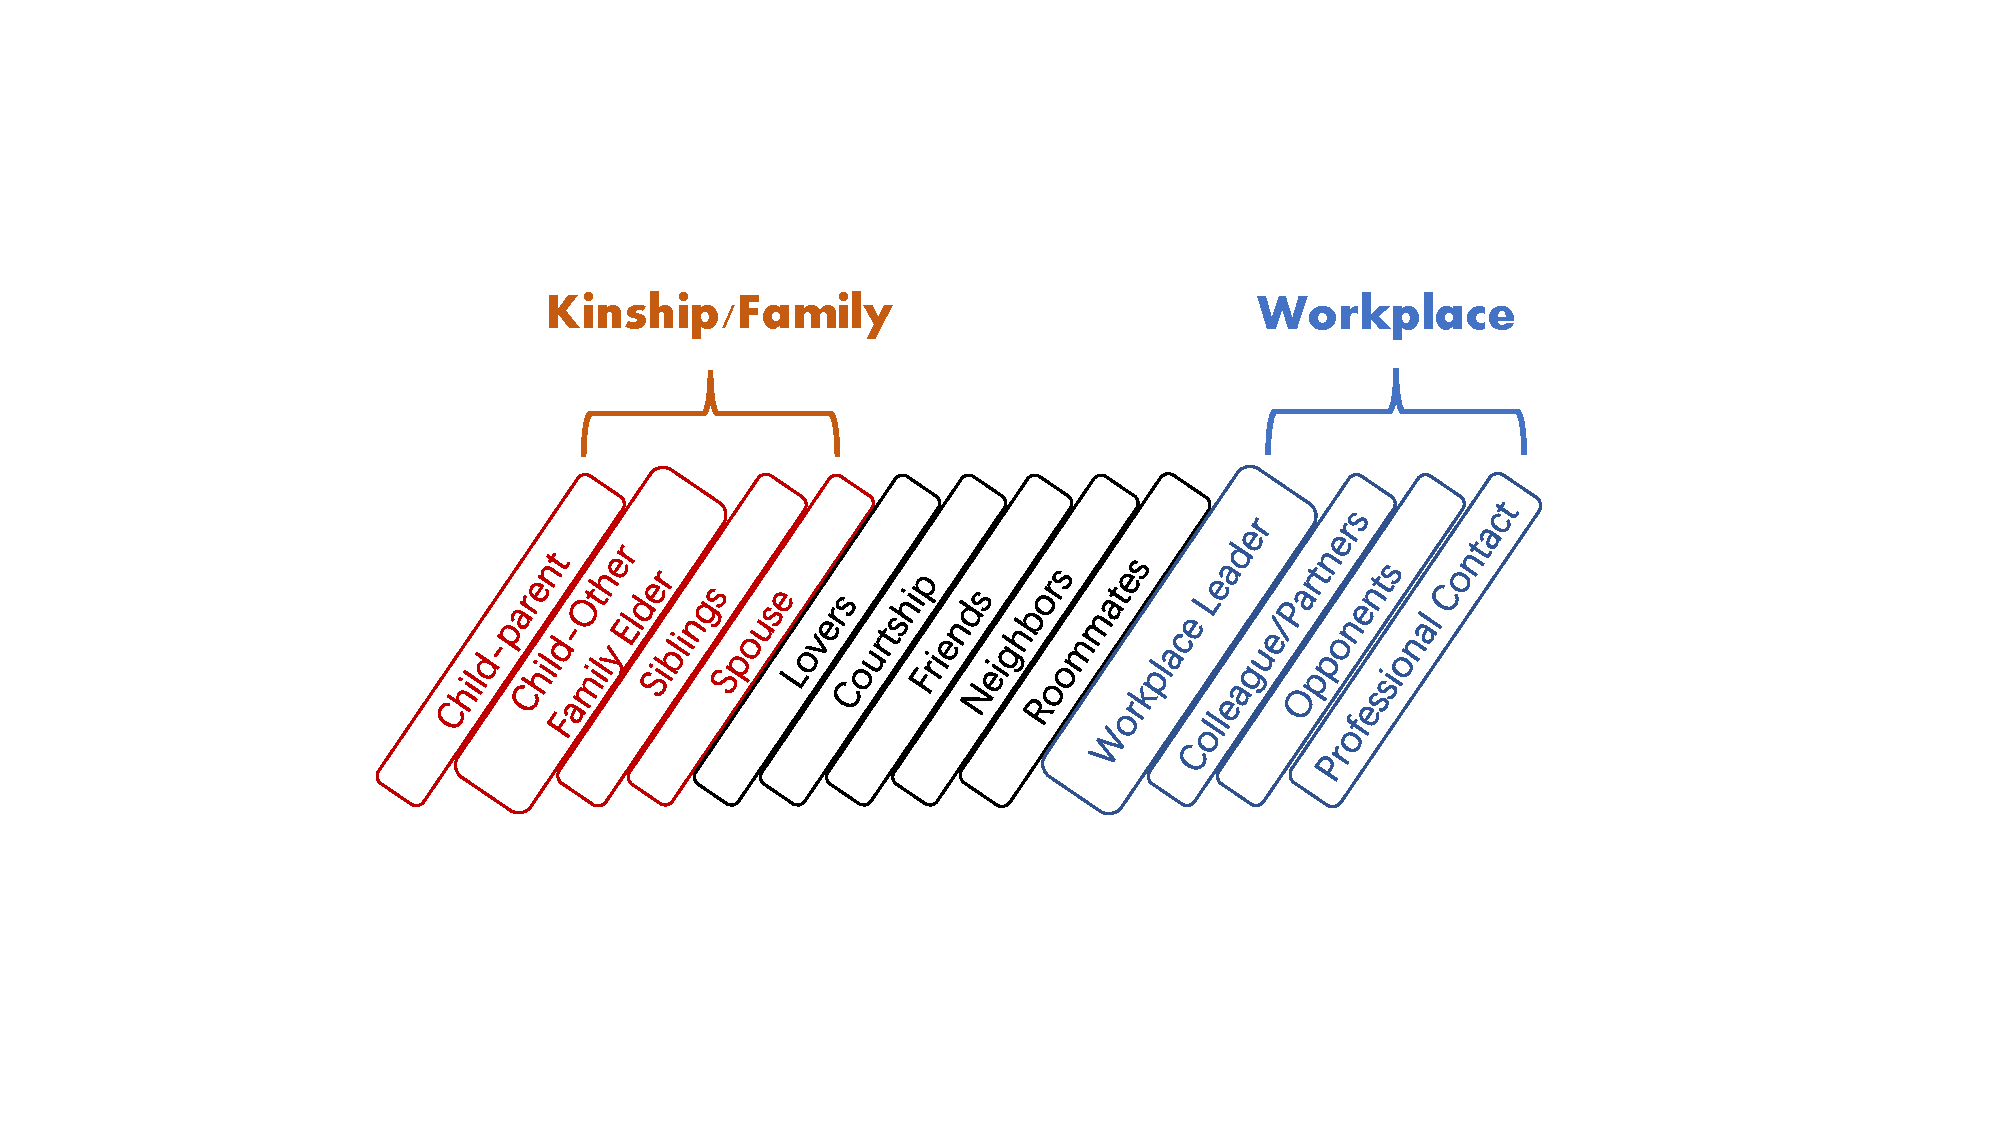
\includegraphics[width=0.99\columnwidth]{taxonomy.pdf}
	\caption{Our 13-class taxonomy of relationships. 
The family and workplace relationships are two groups of 
fine-grained relationships inside the colored frames.}
	\label{fig:taxonomy}
\end{figure}
An important social psychology problem concerned in our task is 
how to classify personal relationships. A taxonomy of personal 
relationships has been considered as a prerequisite for 
understanding their functionalities and 
social effects~\cite{taxonomy2}. 
There are many discussions on this, a great deal of 
which describe relationships by certain 
characteristics that the researchers believe have social significance, 
such as attachment, intimacy, communalty and independence~\cite{class-SDT, encyclopedia}. For example, \citeauthor{class1} 
classified relationships into ``communal'' ones and ``exchange'' ones by 
the rules governing the giving and receiving. 
A problem with those taxonomies is the characteristics 
are very domain-specific~\cite{taxonomy2}, 
which means the label-obtaining process would require highly 
professional annotators, and the results only pertain to
certain topics and say little about others. 
Therefore, in this paper we adopt a taxonomy that makes 
more general sense in life: classify relationships by their 
relatively objective social connections such as child-and-parent, 
spouse and co-workers. 
Although individual difference exists in every real-world case, 
it was found that  each relationship category has different expectations, 
special properties (e.g., marriage usually involves sex, 
shared assets and the production of children)~\cite{class-property}, 
distinctive activities (e.g., talking, eating, drinking and 
joint leisure for friendship) and 
rules~\cite{class-rules} of its own, which are agreed across cultures.

We define a 13-class taxonomy of relationships
(illustrated in \figref{fig:taxonomy}) 
based on \citeauthor{encyclopedia}'s book, 
in which they elaborate on psychological 
and social aspects of various relationships. 
Note that this is not an all-round coverage of 
all possible relationships in human society, 
but an attempt to summarize those common ones.

\subsubsection*{Annotation}
Although personal relationships are not static or mutual exclusive, 
most of them exhibit relative stability over time~\cite{stability}, and
 relationships in movies are usually more clearcut. 
Therefore, in this paper, we model relationship as a single, 
stable label. Such assumption simplifies our task and 
significantly reduces the workload of labeling, though it introduces 
ambiguity in certain cases such as varing relationships 
(e.g., courtship $\rightsquigarrow$ lover $\rightsquigarrow$ spouse) or 
concurrent ones that do not usually exist together
(e.g., enemies falling in love). To avoid these situations, We require the annotator to only 
assign labels when the relationship is clear, relatively stable and typical.

Our groundtruth annotator was provided with the movie title, 
the pair of characters involved in the dialogue, 
movie synopsis from IMDb and Wikipedia for each movie, 
as well as complete access to the Internet, 
and was asked to choose between one out of 13 classes or 
``Not applicable (NA)'' label. 

It took the annotator 100 hours across one and a half months to 
finish the annotation of 300 movies, at a rate of approximately 
$4.07$ minutes per pair. Only $47.11\%$ of the pairs
received a specific label, while others are considered ``not applicable''. 
A detailed statistical description of our current dataset 
along with annotaion evaluation is provided in \secref{sec:eval}.

